\documentclass{article}

% if you need to pass options to natbib, use, e.g.:
\PassOptionsToPackage{numbers, compress}{natbib}
% before loading neurips_2024


% ready for submission
% \usepackage{neurips_2024}


% to compile a preprint version, e.g., for submission to arXiv, add add the
% [preprint] option:
\usepackage[preprint]{neurips_2024}
% to compile a camera-ready version, add the [final] option, e.g.:
%     \usepackage[final]{neurips_2024}


% to avoid loading the natbib package, add option nonatbib:
% \usepackage[nonatbib]{neurips_2024}


\usepackage[utf8]{inputenc} % allow utf-8 input
\usepackage[T1]{fontenc}    % use 8-bit T1 fonts
\usepackage{hyperref}       % hyperlinks
\usepackage{url}            % simple URL typesetting
\usepackage{booktabs}       % professional-quality tables
\usepackage{amsfonts}       % blackboard math symbols
\usepackage{nicefrac}       % compact symbols for 1/2, etc.
\usepackage{microtype}      % microtypography
\usepackage{xcolor}         % colors
\usepackage{ctex}           % 中文支持
\usepackage[numbers]{natbib}  
\usepackage{graphicx}
\title{通过高效微调与数据增强提高大语言模型数学推理能力}


% The \author macro works with any number of authors. There are two commands
% used to separate the names and addresses of multiple authors: \And and \AND.
%
% Using \And between authors leaves it to LaTeX to determine where to break the
% lines. Using \AND forces a line break at that point. So, if LaTeX puts 3 of 4
% authors names on the first line, and the last on the second line, try using
% \AND instead of \And before the third author name.


\author{%
  游年浩\thanks{这些作者贡献相同}\\
  复旦大学 \\
  上海市杨浦区邯郸路220号 \\
  \texttt{nhyou21@m.fudan.edu.cn} \\
  \And
  宋文彦\footnotemark[1]\\
  复旦大学 \\
  上海市杨浦区邯郸路220号 \\
  \texttt{wysong21@m.fudan.edu.cn} \\
  \And
  钟思祺\footnotemark[1]\\ 
  复旦大学 \\
  上海市杨浦区邯郸路220号 \\
  \texttt{sqzhong21@m.fudan.edu.cn} \\
}


\begin{document}


\maketitle


\begin{abstract}
  在自然语言处理(NLP)领域,大型语言模型(LLMs)在多种任务中展现出卓越性能,其中包括数学推理。然而,数学推理任务中的错误可能导致整个解决过程的破坏。为了提升LLMs的数学推理能力,研究者通常在监督推理数据集上进行微调。本研究探讨了在有限模型参数规模和计算资源条件下,如何通过高效微调和数据增强提高小型LLM的数学推理性能。我们发现,低秩近似(LoRA)训练、数据集增强和前缀调优(Prefix-Tuning)等方法能够在不显著增加计算成本的情况下,有效提升模型的推理能力。实验结果显示,数据增强方法在GSM8K和MATH数据集上的准确率分别达到了37.07\%和8.00\%,而Prefix-Tuning方法在这两个数据集上的准确率分别达到了57.47\%和11.40\%,相较于基准实验有显著提升。本研究不仅为未来研究提供了新的方向,也为资源受限的挑战提供了务实的解决方案。
\end{abstract}


\section{引言}
\label{sec:introduction}
在自然语言处理(NLP)领域,大型语言模型(LLMs)\citep{ouyang2022traininglanguagemodelsfollow, anil2023palm, raffel2023exploringlimitstransferlearning},在各种任务中表现出卓越的性能,包括文本分类\citep{min-etal-2022-metaicl,pmlr-v202-jiang23k,devlin-etal-2019-bert}、代码生成\citep{wei2024magicoderempoweringcodegeneration}、指令跟随\citep{zhou2023instructionfollowingevaluationlargelanguage,lei2024instructercreformingemotionrecognition}和数学推理\citep{DBLP:conf/nips/Wei0SBIXCLZ22, taylor2022galacticalargelanguagemodel, lewkowycz2022solvingquantitativereasoningproblems}。在这些任务中,处理数学推理的能力已成为评估不同LLMs能力的典型且重要的标准\citep{cobbe2021training,hendrycks2021measuring}。然而,数学推理任务中面临的一个主要挑战是,即便是一个轻微的错误也可能破坏整个解决过程\citep{Lightman2023LetsVS}。

通常,为了增强LLMs的数学推理能力,研究人员会在监督推理数据集上进行微调。为提高开源LLMs的数学推理能力,一系列工作应用于这一领域,其中一种主流方法是先扩充新的数学问题和答案,然后在增强数据集上进行监督微调\citep{yuan2023scalingrelationshiplearningmathematical, luo2023wizardmathempoweringmathematicalreasoning, yu2024metamathbootstrapmathematicalquestions},这种方法已经取得了良好的结果。然而,在有限的模型参数规模(如0.5亿参数)和计算资源条件下,微调小规模LLM以提升数学推理性能依然存在以下挑战:
(1) 模型规模限制:小规模的模型可能缺乏足够的参数来有效捕捉复杂的数学推理关系。
(2) 数据稀缺性:高质量的数学推理数据集相对稀少,这限制了模型的训练效果。
(3) 计算资源限制:有限的硬件资源限制了长时间、大规模的训练过程,且可能不适合现有的大型数据集。

在对现有方法和模型的评估中,我们发现虽然大型语言模型在数学推理方面取得了显著进展,但其在处理复杂数学问题时仍常出现不足。具体来说,模型在推理过程中容易面临以下问题:对问题背景的理解不够深入,缺乏将多个步骤有效连接的能力\citep{Huang_2024},以及在面对不熟悉或新颖问题时表现出不稳定性。这些问题突显出当前模型在表达和推理能力上的局限。加之,相较于其他自然语言处理任务,数学推理任务需要对数量信息和逻辑关系有更深刻的理解和处理能力,这为模型设计和训练提出了更高的要求。

尽管在许多任务中通过扩展训练数据集已被验证为一种有效的提升手段\citep{tao2024survey},但数学推理任务的数据集仍较为稀缺且难以构建。这些因素都增加了训练和微调过程的复杂性,尤其是在资源有限的情况下。因此,需深入分析如何在小参数规模和有限算力资源下,优化模型的数学推理能力,以实现性能的进一步提升。考虑到这些因素,我们的研究旨在通过诸多创新性方法和策略来克服这些挑战。

基于这些挑战,我们的研究提供了以下见解:(1) LoRA训练:通过运用低秩近似技术调节模型参数,这种方法能够显著降低计算开销,使其适合于资源有限的场景。我们发现这种方法在保持模型性能的同时减少了计算资源的消耗。(2) 数据集增强:通过扩展和丰富数学推理数据集,可以有效提升模型的泛化能力,使其更好地应对多样化的问题情境。这一策略不仅增强了模型对已知问题的处理能力,也提高了其解决新问题的潜力。(3) Prefix-Tuning:此方法通过为输入提供特定前缀进行优化,提供了一种灵活整合额外知识的途径,而无需对模型的大规模参数进行调整。它为模型在动态环境下的适应能力提供了支持。

通过对上述方法的仔细分析,我们进一步认识到,结合这些技术可以在不增加过多计算负担的情况下,有效地增强模型的推理能力。这些见解不仅为未来的研究提供了新的方向,也为应对资源受限的挑战提供了务实的解决方案。

我们的贡献包括:  

\begin{itemize}  
    \item 完成了Qwen2.5-0.5B SFT的测试,结果显示在GSM8K和MATH上的准确率表现分别为34.27\%和7.00\%。
    \item 详细探索和验证了一系列在受限环境下微调LLM的策略,创新性地应用了LoRA、数据增强和Prefix-Tuning方法,在有限的参数规模和计算资源条件下,实现了对标准模型的显著性能提升。
    \item 数据增强方法在GSM8K和MATH上准确率分别达到了37.07\%和8.00\%,Prefix-Tuning方法在GSM8K和MATH上准确率分别达到了57.47\%和11.40\%,对比基准实验有显著提升,证明其在实际应用中的可行性。
\end{itemize}
\section{相关工作}
\label{sec:relatedwork}

\textbf{大型语言模型的数学推理  } 大型语言模型的数学推理能力是一个关键能力\citep{yuan2023well}。通过数学相关的预训练\citep{lightman2023let}和数学相关的监督微调\citep{yu2024metamathbootstrapmathematicalquestions},LLM的数学推理能力可以得到增强。为了通过监督微调提升数学推理能力,这种方法通常涉及利用更大规模的模型或手动收集高质量数据\citep{tao2024survey}。MetaMath\citep{yu2023metamath}通过重写数学查询并在LLM的帮助下提供答案来扩展其数据集。MAmmoTH\citep{yue2309mammoth}编制了多样化的数学数据集用于训练,通过包含推理的思维链(CoT)和思维程序(PoT)推理理由来丰富数据集,从而形成了MathInstruct数据集。RFT\citep{yuan2023scaling}是一种标准在线RL的简化离线方法。它通过SFT模型生成和收集准确的推理路径来增强其训练数据集。

\textbf{思维链推理 } 语言模型多步推理的重要方法是由Wei等人\citep{wei2022chain}提出的思维链提示。他们指出,推理能力只能通过思维链触发,而不是通过直接给出答案的标准提示。后续研究表明,思维链可通过自我一致性\citep{wang2022self}、latex格式的数据预训练\citep{lewkowycz2022solving}、上下文选择\citep{creswell2022selection},甚至添加短语“Let’s think step by step”\citep{kojima2022large}得到改进。原始CoT论文使用8个手动编写的示例作为提示,这些示例被大多数后续研究采用。

\textbf{大型语言模型的数据增强 }  数据增强是提高NLP下游任务表现的常用技术\citep{feng-etal-2021-survey}。在大型语言模型时代,数据增强通常用于生成遵循指令的SFT数据集\citep{wang-etal-2023-self-instruct}。SFT数据集的查询和响应\citep{ding2023enhancing}都可以通过提示最先进的专有LLM进行增强。


\section{方法}
\label{sec:methodology}
在本研究中,我们旨在探讨预训练语言模型在特定的数学任务上的应用潜力,特别是通过结合不同的微调技术和数据增强策略来优化模型性能。我们的目标是有效利用现有资源,在不显著增加计算成本的前提下,测试Qwen2.5系列模型\citep{qwen2.5}的表现。我们以Qwen2.5-0.5B的监督微调为一个稳健的基线模型,然后依次探索低秩适应(LoRA)、前缀调优(Prefix Tuning)等参数高效微调技术,以及反思增强(Reflective Augmentation)等数据扩充方法的效果。此外,我们还将评估专家模型在资源受限条件下的表现,以全面了解参数量和数据类型对模型性能的影响。
\subsection{基线模型微调}
\textbf{监督微调与基线建立。} 我们首先构建了一个基线模型,该模型基于Qwen2.5-0.5B,并分别在GSM8K\citep{cobbe2021training}和MATH\citep{hendrycksmath2021}两个数据集上进行了监督微调(Supervised Fine-Tuning, SFT)。这两个数据集分别聚焦于基础算术问题解决能力和高等数学推理能力,为模型提供了全面而深入的学习材料。

\subsection{参数高效微调}
\textbf{低秩适应(Low-Rank Adaptation, LoRA)。} 为了在有限计算资源下提升模型性能,我们引入了低秩适应(LoRA)技术 \citep{hu2022lora}。LoRA通过仅更新预训练模型权重矩阵的低秩近似部分来减少需要调整的参数数量,从而降低内存和计算需求,同时提高特定任务上的性能。这种方法特别适合资源受限环境。

\textbf{前缀调优(Prefix Tuning)。} 我们还应用了前缀调优(Prefix Tuning)技术 \citep{li2021prefixtuning} 来改进微调效率。前缀调优通过在输入序列前添加可训练的前缀向量,引导模型生成符合新任务需求的输出,而不直接修改原模型参数。这种方法减少了训练时间和显存占用,避免了灾难性遗忘,并允许模型灵活适应多种下游任务。。

\subsection{查询(Query)和响应(Response)增强与数据扩充}
\textbf{查询响应增强以扩充数据集。} 在探索提升数学推理任务中大型语言模型的性能时,我们意识到数据增强是提高模型泛化能力的关键。因此,我们应用了Li\citep{li2023query}提出的数据增强技术,通过演化查询(query evolution)和多样化推理路径来扩充数据集。这种方法不仅增加了数据集的规模,而且通过引入更复杂和多样化的问题表述以及多个推理路径,创建了两个新数据集AugGSM8K和AugMATH,提高了数据的质量。我们在这些扩充数据集上进行的监督式微调进一步优化了性能。

\subsection{专家模型}
\textbf{模型的选择。} 尽管理想情况下我们希望对更大规模的模型进行全面微调,但实际操作中却面临着设备显存等硬件资源的限制。为此,我们特别选择了Qwen2.5-MATH-1.5B这一专门为数学领域优化的模型进行实验。该模型不仅拥有更多的参数量,而且是在一个更为专业的数学数据集上训练而成,这使得我们可以探讨参数量和数据类型对于预训练模型性能的具体影响。
\section{实验}
\label{sec:experiments}

\subsection{实验设计}

\textbf{数据集。} 本实验选取了两个具有代表性的数学问题数据集:GSM8K\citep{cobbe2021training}和MATH\citep{hendrycksmath2021}。GSM8K数据集由OpenAI发布,包含8.5K个小学数学问题,这些问题覆盖了基础的算术运算,适合用来评估模型对基础数学问题的处理能力。MATH数据集则由加州大学伯克利分校的研究团队开发,包含12,500个来自高中数学的问题,这些问题的难度更高,覆盖了更广泛的数学领域,适合用来评估模型对较复杂数学问题的推理能力。在本实验中,测试集分别为GSM8K的test子集,以及MATH500子集,以便于对比和分析。

\textbf{模型。} 实验中主要使用了Qwen2.5系列模型\citep{qwen2.5},这是一个基于LLM(Large Language Models)的模型家族,提供了不同规模的模型以适应不同的计算资源和任务需求。具体来说,我们使用了0.5B和1.5B两种规模的模型进行实验。这些模型均在Hugging Face平台上提供,便于进行微调和部署。

\textbf{实验环境配置。} 
为了确保实验结果的可靠性并且提高实验的效率,本研究在最终实验阶段租用了AutoDL平台的服务器,使用了如下配置的计算平台进行实验:
\begin{itemize}
    \item \textbf{硬件配置}:
        \begin{itemize}
            \item \textbf{图形处理单元 (GPU)}: NVIDIA GeForce RTX 4090, 24GB GDDR6X 
            \item \textbf{中央处理器 (CPU)}: Intel (R) Xeon (R) Platinum 8481C,16 CPU
            \item \textbf{内存}: 80GB RAM
        \end{itemize}
    \item \textbf{软件配置}:
        \begin{itemize}
            \item \textbf{操作系统}: Ubuntu 22.04 LTS
            \item \textbf{编程语言}: Python 3.12
            \item \textbf{深度学习框架}: PyTorch 2.5.1
            \item \textbf{CUDA 版本}: CUDA Toolkit 12.4 \end{itemize}
\end{itemize}

\subsection{实验结果} 

\begin{figure}[htbp]
    \centering
    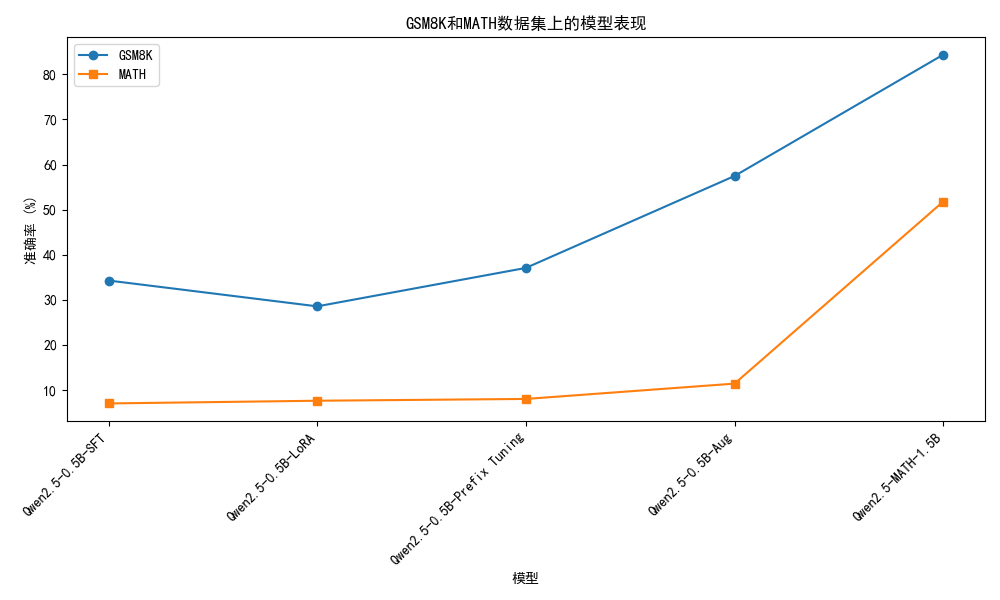
\includegraphics[width=0.9\textwidth]{figs/model_acc.png} 
    \caption{不同方法在GSM8K和MATH数据集上的准确率对比}
    \label{fig:experiment_result}
\end{figure}

\textbf{主要结果。} 
 表格\ref{fig:experiment_result}总结了各个模型在 GSM8K 和 MATH 数据集上的准确率。结果显示,在 GSM8K 数据集上,Qwen2.5-0.5B-SFT、Qwen2.5-0.5B-LoRA、Qwen2.5-0.5B-Prefix Tuning、Qwen2.5-0.5B-Aug 和 Qwen2.5-MATH-1.5B的生成结果分别达到了34.27\%、28.54\%、37.07\%、57.47\%和84.38\%的准确率;而在 MATH 数据集上,分别达到了7.00\%、7.60\%、8.00\%、11.40\%和51.80\%的准确率。

\textbf{不同方法的影响}
\begin{itemize}
    \item \textbf{监督微调(SFT)}:作为基线模型,SFT 展示了模型在简单训练的情况下处理数学问题的能力,参数量仅仅0.5B的模型在SFT后即可完成一部分简单数学题目,在GSM8K和MATH数据集上准确率分别为34.27\%和7.00\%,在实验环境中训练用时合计约60分钟。
    \item \textbf{LoRA 技术}:通过使用 LoRA 进行微调,我们观察到相比于 SFT,在在 GSM8K 数据集上准确率下降了 5.73\%,而在 MATH 数据集上准确率提高了 0.6\%。这可能是由于 LoRA 的参数高效特性限制了模型学习新知识的能力,特别是在面对求解数学题这一复杂任务时。然而,LoRA 的优势在于显著减少了计算资源的需求,使得大规模模型的微调成为可能,在实验环境中训练用时合计约20分钟。
    \item \textbf{Prefix Tuning技术}:Prefix Tuning展示了其卓越的适应能力。由于Prefix Tuning只引入了额外的前缀向量,不会改变原始模型参数,可以缓解传统微调过程中的灾难性遗忘问题,提高性能。实验结果显示,Prefix Tuning不仅在资源受限条件下缩短了训练时间和显存占用,在GSM8K和MATH数据集上,Prefix Tuning的表现均优于完全微调的基线模型,分别提升了23.20\%和4.40\%。在实验环境中,Prefix Tuning的训练用时合计约40分钟。
    \item \textbf{查询响应增强}:查询响应增强技术通过引入更复杂和多样化的问题表述以及多个推理路径,显著提升了数据集的质量和多样性。这种方法促进了模型对问题更深层次的理解。实验结果表明,应用查询响应增强后的模型在复杂数学推理任务上表现略有提升,在GSM8K和MATH数据集上的准确率分别提升了2.80\%和1.00\%,但是数据量较大,在实验环境中训练用时合计约180分钟。
    \item \textbf{MATH专家模型}:针对资源受限的情况,我们选择了专门为数学领域优化的大模型Qwen2.5-MATH-1.5B进行测试。实验显示,该模型在增加了参数量,而且在专业数学数据集上进行了预训练的情况下,在数学推理任务上展现了极高的准确率,在GSM8K和MATH数据集上的准确率分别提升了50.11\%和44.80\%,达到了84.38\%和51.80\%。该模型未在本地进行训练。
\end{itemize}

\subsection{结果分析} 
\subsubsection{高效微调与数据增强的性能影响分析}

高效微调技术在资源受限条件下的应用展现了显著的优势。LoRA在计算资源消耗上性能优越,然而其在GSM8K数据集上性能下降的现象揭示了这样一种可能:在任务的复杂性和需要捕捉的知识结构较为动态的场景中,LoRA的表达能力可能受限。这限制了其在复杂推理任务中的适应性和灵活性。

相比之下,Prefix Tuning技术展示了其优越的适应能力。这种方法有效地缓解了灾难性遗忘问题,在不增加计算复杂度的同时,提升了模型在新任务上的性能表现。在GSM8K和MATH数据集上的卓越表现说明,Prefix Tuning不仅保留了基础模型的知识架构,还为模型理解和应对高度复杂的推理任务提供了强有力的支持。

在数据增强方面,查询响应增强策略通过复杂化输入问题和多样化推理路径,提升了模型训练数据集的多样性和质量。这一方法增强了模型在复杂数学推理任务中的理解深度和泛化性能,但也增加了学习负担,训练时间翻倍。实验结果显示,尽管准确率略有提升,但在小模型参数规模下,数据增强对模型推理能力的提升有限,因模型对数据的理解能力本身受限。

\subsubsection{GSM8K vs. MATH 性能差异} 
从整体上看,模型在 GSM8K 上的表现明显优于 MATH 数据集。这一现象可以归因于两个数据集的性质差异:GSM8K 主要包含小学级别的基础算术运算问题,而 MATH 则涵盖了高中水平的复杂数学概念和推理问题。因此,MATH 数据集对模型提出了更高的要求,不仅需要理解复杂的数学符号和术语,还需要进行多步逻辑推理。这种复杂性增加了模型出错的概率,从而导致了较低的准确率。值得注意的是,MATH 数据集在 MATH 专家模型方法下的提升幅度明显高于 GSM8K 数据集,可能是因为该方法的大模型 Qwen2.5-MATH-1.5B 专为数学领域优化并在专业数学数据集上预训练,能够更有效地处理复杂的数学概念和推理任务。这种专门的优化使得模型对 MATH 数据集的复杂性具有更强的适应能力,从而显著提升准确率。

\section{限制与讨论}
\label{sec:limitation}尽管我们在提高开源 LLMs 数学推理能力方面取得了积极成果,但仍存在一些局限性。首先,由于计算资源的约束,未能对更大规模的模型进行全面测试,这可能影响了模型性能的最大化。其次,我们的研究主要集中在基础至中等难度的数学问题上,对于模型处理高级别复杂数学推理的能力仍有待深入探讨。此外,虽然我们提出的方法展示了良好的效果,但对于不同类型数学问题的有效性和泛化能力还需要更多的实证支持。

未来的研究可以从以下几个方向展开:一是继续扩大实验模型的规模,二是探索更多类型的数学问题以评估模型的广度和深度,三是开发更先进的数据增强和微调技术,四是考虑将外部工具如计算器或符号计算系统集成到模型中,以辅助解决更复杂的数学问题。
\section{结论}
\label{sec:conclusion}
本研究表明,在资源受限的情况下,结合参数高效微调技术和数据增强策略可以有效提升 LLMs 的数学推理能力。此外,专家模型的使用进一步验证了大规模、特定领域优化模型在复杂任务上的优越性。这些发现不仅为未来的研究提供了新的方向,也为实际应用中的模型优化提供了务实的解决方案。尽管如此,进一步扩大实验模型规模、探索更多类型数学问题以及开发更先进的微调技术仍然是未来研究的重要方向。通过这些努力,希望能促进人工智能在数学教育和其他应用场景中的应用。

\bibliographystyle{ACM-Reference-Format}
\bibliography{ref}

\appendix
\section{个人贡献}
\label{sec:personalcontribution}

\textbf{组长 游年浩(21302010043)} 
\begin{itemize}  
    \item 对于Qwen2.5-0.5B模型针对数学推理任务展开\textbf{其他模型}的调研,尝试Qwen2.5-MATH-1.5B在gsm8k和MATH数据集上进行测试。
    \item 完成\textbf{方法}、\textbf{实验}、\textbf{限制与讨论}、\textbf{结论}部分的写作。
\end{itemize}

\textbf{组员 宋文彦(21302010062)} 
\begin{itemize}  
    \item 对于Qwen2.5-0.5B模型针对数学推理任务展开微调方法的调研,除SFT外尝试Lora、Prefix Tuning微调,在gsm8k和MATH数据集上进行训练和测试。
    \item 完成\textbf{个人贡献}部分的写作。
\end{itemize}

\textbf{组员 钟思祺(21302010069)} 
\begin{itemize} 
    \item 对于Qwen2.5-0.5B模型针对数学推理任务展开数据增强方法的调研,尝试用AugMATH、AugGSM8K数据集进行微调,在gsm8k和MATH数据集上进行测试。
    \item 完成\textbf{引言}、\textbf{相关工作}、\textbf{实验}部分的写作。
\end{itemize}

\end{document}